\documentclass[12pt, a4paper]{article}
\usepackage[utf8]{inputenc} 
\usepackage[english]{babel}
\usepackage{latexsym}
\usepackage{url}
\usepackage{fancyhdr}
\usepackage{hyperref}
\usepackage{xparse}
\usepackage{graphicx}
\usepackage{amssymb}
\usepackage{multirow}
\usepackage{color}
\usepackage{pmboxdraw}

\usepackage{fancyvrb}
\usepackage{xcolor}

% to include the code
\usepackage{listings}
\usepackage{color}

% appendix
\usepackage[toc,page]{appendix}

\usepackage{mathtools}


\definecolor{mygreen}{rgb}{0,0.6,0}
\definecolor{mygray}{rgb}{0.5,0.5,0.5}
\definecolor{mymauve}{rgb}{0.58,0,0.82}

\lstset{ %
  backgroundcolor=\color{white},   % choose the background color
  basicstyle=\footnotesize,        % size of fonts used for the code
  breaklines=true,                 % automatic line breaking only at whitespace
  captionpos=b,                    % sets the caption-position to bottom
  commentstyle=\color{mygreen},    % comment style
  escapeinside={\%*}{*)},          % if you want to add LaTeX within your code
  keywordstyle=\color{blue},       % keyword style
  stringstyle=\color{mymauve},     % string literal style
}



\DeclarePairedDelimiter\ceil{\lceil}{\rceil}
\DeclarePairedDelimiter\floor{\lfloor}{\rfloor}


\title{SAD calculation of two monochrome images}
\author{Francesco Urbani}
\date{\today}



\frenchspacing
\pagestyle{fancy}
\fancyhf{}
\rhead{\bfseries\thepage}


\renewcommand{\sectionmark}[1]{\markboth{\thesection.\ #1}{}}

\setcounter{section}{-1}

\begin{document}
\maketitle

\newpage
\tableofcontents

\newpage 
\listoffigures
\newpage

\section{Project specifications}


Design a synchronous digital system that calculates the SAD value, defined as the sum of the magnitude of the differences of each pixel of two (monochrome) images, image A and image B. Each pixel's value is stored in \texttt{N}-bits and each image has \texttt{px} pixels per side.

The circuit has a \textit{clock}, a \textit{reset} and an \textit{enable} signal as inputs together with the signals \textit{PA} and \textit{PB} representing one pixel of each image flowing into the system from the outside, sequentially.
The circuit has a \texttt{M}-bits output signal called \textit{SAD} where:

\begin{equation}
    2^\texttt{M} \ge (2^\texttt{N}-1) \cdot \mbox{\texttt{px}}^2
\end{equation}

and a \textit{DATA\_VALID} signal which is set when the SAD calculation is completed.

When the reset is active, \textit{SAD} and \textit{DATA\_VALID} are 0. If the enable signal is zero the system does not change its current state.



\newpage

\section{Introduction}

In digital image processing, the sum of absolute differences (SAD) is a measure of the similarity between image blocks. It is calculated by taking the absolute difference between each pixel in the original block and the corresponding pixel in the block being used for comparison. These differences are summed to create a simple metric of block similarity, the L1 norm of the difference image or Manhattan distance between two image blocks.

The sum of absolute differences may be used for a variety of purposes, such as object recognition, the generation of disparity maps for stereo images, and motion estimation for video compression.
\newline

The sum of absolute differences provides a simple way to automate the searching for objects inside an image, but may be unreliable due to the effects of contextual factors such as changes in lighting, color, viewing direction, size, or shape. The SAD may be used in conjunction with other object recognition methods, such as edge detection, to improve the reliability of results.


\subsection{State of the art architectures}

\begin{itemize}
\item Implementation of SAD Algorithm with Folded Tree Architecture using VHDL\\
(\href{http://www.internationaljournalssrg.org/IJECE/2015/Volume2-Issue7/IJECE-V2I7P107.pdf}{\texttt{http://www.internationaljournalssrg.org/IJECE/2015/Volume2\-Issue7/IJECE\-V2I7P107.pdf}})

\item A Highly Parallel SAD Architecture for Motion
Estimation in HEVC Encoder \\
\href{http://unitec.researchbank.ac.nz/bitstream/handle/10652/3813/PID3380667.pdf}{\texttt{http://unitec.researchbank.ac.nz/bitstream/handle/10652\\/3813/PID3380667.pdf}}

\end{itemize}



\newpage
\section{Algorithm description}


The two images are fed into the system by means of two signals, called \textit{PA} and \textit{PB}, whose size is \texttt{N}, i.e. the number of bits representing the pixel grade on a scale from 0 (i.e. 100\% black) to $2^N-1$, typically 255 (i.e. 100\% white).

Being the system synchronous, it works on the clock rising-edge.


The other two inputs are the \textit{reset} (active high) and the \textit{enable}, that prevents the SAD value from being updated when it's on its low state.

The two outputs are \textit{SAD} and \textit{DATA\_VALID}. 

\textit{SAD} represent the actual information we are interested in, and it's defined as the sum of the absolute differences of each pixel of the two images. 
Therefore it's value is updated at each clock-cycle and it is only frozen whenever the \textit{enable} is low or the calculation is completed.

\textit{DATA\_VALID} goes high when the SAD calculation is finished and it stays high until a reset occurs.






%\newpage
\section{Architecture}

The following is a basic architecture representation of the algorithm just described, with the wires labeled according to the specific case\\ 
\texttt{N}=8, \texttt{px}=16 ($\Rightarrow$ \texttt{SAD\_bits}=16),\\ 
but can be extended to any number of bits, later in the code.
\newline



\begin{figure}[h]
\centering
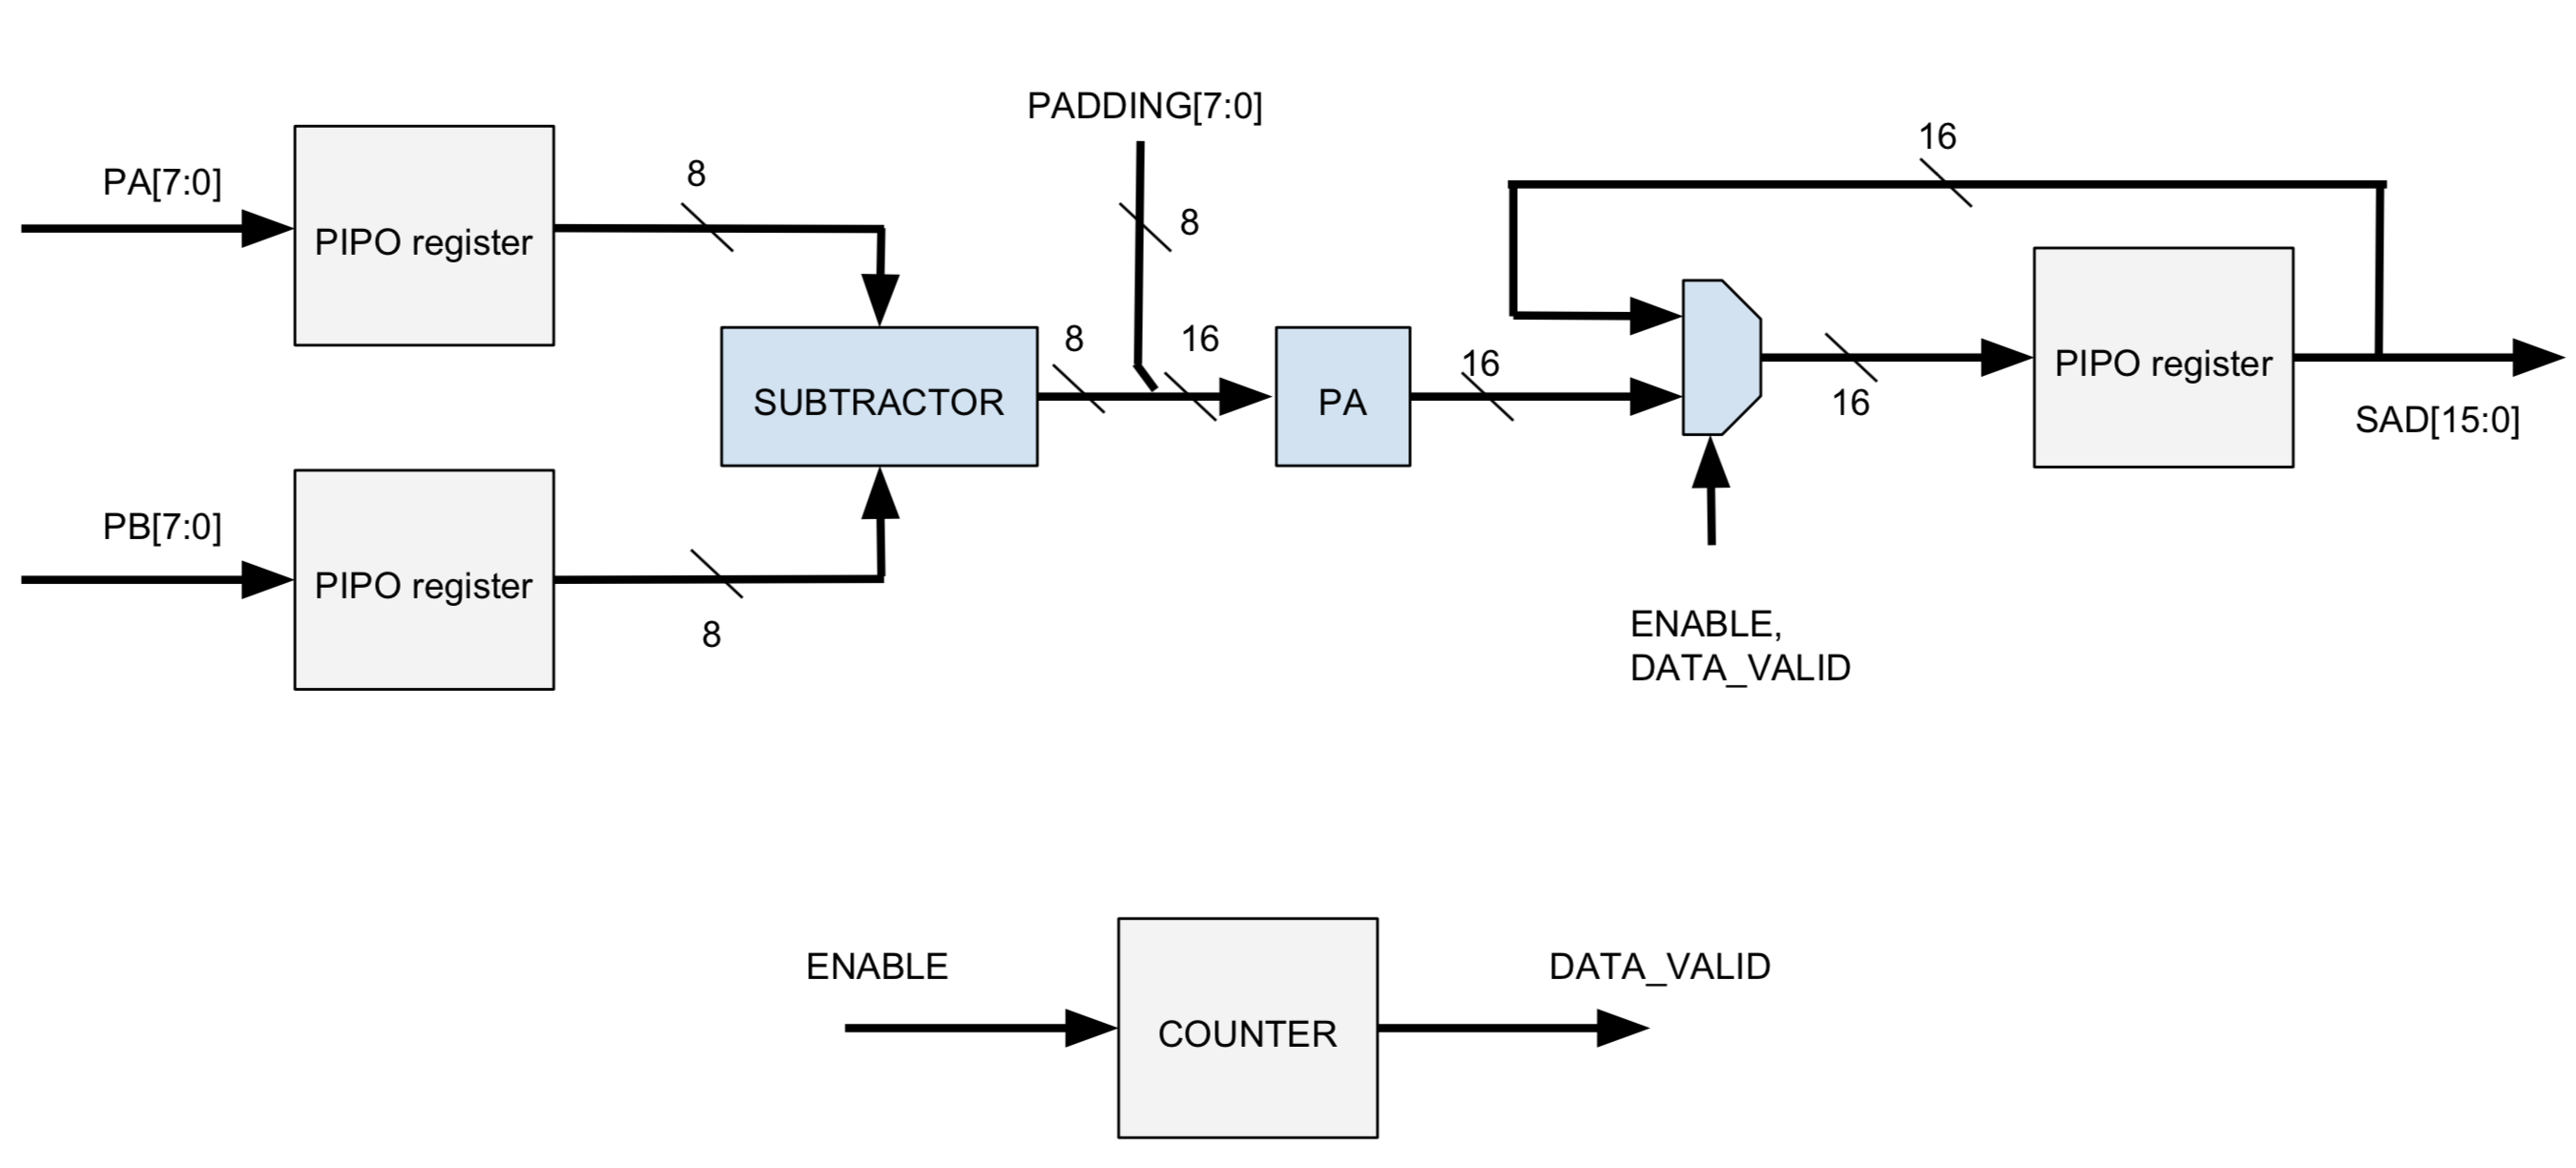
\includegraphics[scale=0.3]{../screenshots/arch1.png}
\caption{Architecture diagram}\label{fig:7}
\end{figure}


\subsection{Design choices}

%What has not already being said is the following:

\begin{itemize} 
%\item the reset is active high;


\item the signal \textit{padding} has been necessary to "tune" the upstream signal out of the subtractor to the downstream signal. It's type is \texttt{std\_logic\_vector [SAD\_bits-N-1 downto 0]} and it is \texttt{x"00"} in the default configuration.

\item PA is a phase accumulator;

\item the multiplexer following the PA has the function to freeze the value of the output SAD when it must not be changed, that's why the control signal of the MUX depends upon \textit{enable} and \textit{DATA\_VALID}, more specifically it is
 \texttt{S <= EN nand (not RESET)}, i.e. it lets the signal flow ahead only when \textit{enable} is \texttt{1} and \textit{DATA\_VALID} is \texttt{0};
 
 \item the counter counts up to $\texttt{px}^2$, which means that the whole image has been processed. It then sets its output to 1 until the system is newly reset;
 
 \item the SISO register delays counter enable by 3 clock cycles. This is because 3 clock-cycles is the time displacement between \textit{PA} and \textit{PB} entering the system and \textit{SAD} reacting to those two inputs. 
 Putting a delay on the counter enabler lets the system stay in sync and not erroneously set \textit{DATA\_VALID} to 1 before the actual calculation is completed.
 
 \item since when \textit{enable} is not active the system is required to maintain its state, i.e. being transparent to the input signals \textit{PA} and \textit{PB}, the input reset signal into the "first stage" PIPO registers, is also driven by the \textit{enable} signal, more specifically:

 \texttt{RST\_IN <= EN nand (not RST\_global)}.
 
 

\end{itemize}



\section{VHDL code}

\subsection{Source structure}

A structural approach has been followed.
After writing the \texttt{.vhd} files describing all the components that I would have been using in the top-level one, I've simply wired them up together to create the final design, which is \texttt{SAD.vhd}, see Appendix \ref{appendix:code} for reference.

The only two sub-components described with a \textit{behavioral} approach have been \texttt{counter.vhd} and \texttt{subtractor.vhd}. 

For additional explanation about this section, see the comments along the code (\texttt{./src/*} and \texttt{./tb/*)}.



\subsection{Test benches}

In order to write a meaningful test-bench that would actually test a real-life situation -- meaning that the two images are most likely different from each other pixel by pixel -- writing a script to automate this process turned out to be almost mandatory.

That's right what \texttt{./scripts/tb\_SAD\_generator.py} does: it takes (interactively) as input the number of bits representing each pixel value (\texttt{N}) and the number of pixels/side, i.e. the square root of the total number of pixels composing each image (\texttt{px}), and it calculates beforehand the minimum number of bits necessary to store the SAD value w/o information loss, according to the following expression: 

\begin{equation}
    \ceil[\big]{\ \log_2( (2^\texttt{N}-1) \cdot \texttt{px}^2 )\ } 
\end{equation}
and asks the user whether he wants to increase that number, called \texttt{SAD\_bits}.
\newline

Secondly, the script generates two square matrices with random integer elements in the range $[0, 2^N)$, it calculates a third matrix whose elements are the magnitude of the difference of the former two matrices' elements and eventually it calculates the overall sum of it's elements, i.e. the expected SAD value.
\newline

Eventually it generates/overwrite the test bench file \texttt{./tb/tb\_SAD.vhd} coherently to the model so that comparing the model to the waveform result is a trivial task.
\newline

A second test bench has also been developed first, for a quick debug: two values of PA and PB enters the system without ever changing -- say PA=0; PB=1 -- and checking SAD value to be equal to $\texttt{px}^2$ at the end of the calculation is a preliminary way to check whether the system's working correctly.




\subsection{Compiling instructions}

I've used the open-source compiler \href{http://ghdl.free.fr/}{GHDL} to compile the VHDL code in conjunction with the waveform viewer \href{http://www.logicpoet.com/scansion/}{Scansion} (macOS) which is an alternative to \href{http://gtkwave.sourceforge.net/}{GTKWave} (cross-platform).
\newline

Once organized the folder like this:

\begin{verbatim}
.
├── .work
├── scripts
├── src
├── tb
├── vivado
└── waveforms
\end{verbatim}

move into \texttt{.work/} and from your terminal type:
\newline

\texttt{ghdl -i ../src/*}

\texttt{ghdl -i ../tb/*}
\newline

to import all the \texttt{.vhd} files into the working directory. Then:
\newline

\texttt{ghdl -m sad}
\newline

to compile the top-level component. That will compile all the components 
instantiated into the top-level component as well. Then type:
\newline

\texttt{ghdl -m tb\_sad}
\newline

to compile the test bench of the top-level component. And finally:
\newline

\texttt{ghdl -r tb\_sad --vcd=../waveforms/tb\_SAD.vcd}
\newline

to create the waveform file \texttt{tb\_SAD.vcd} which can be afterwards opened with one of those two above mentioned waveform viewers.





\newpage
\section{Simulations}

\subsection{Simulation 1}

Inputs: \texttt{N}=8; \texttt{px}=16. Number of bits to correctly store \texttt{SAD}=16. This is the default case given by the specification requirements. 

This version is the one that will be later implemented.

\begin{figure}[h!]
%\centering
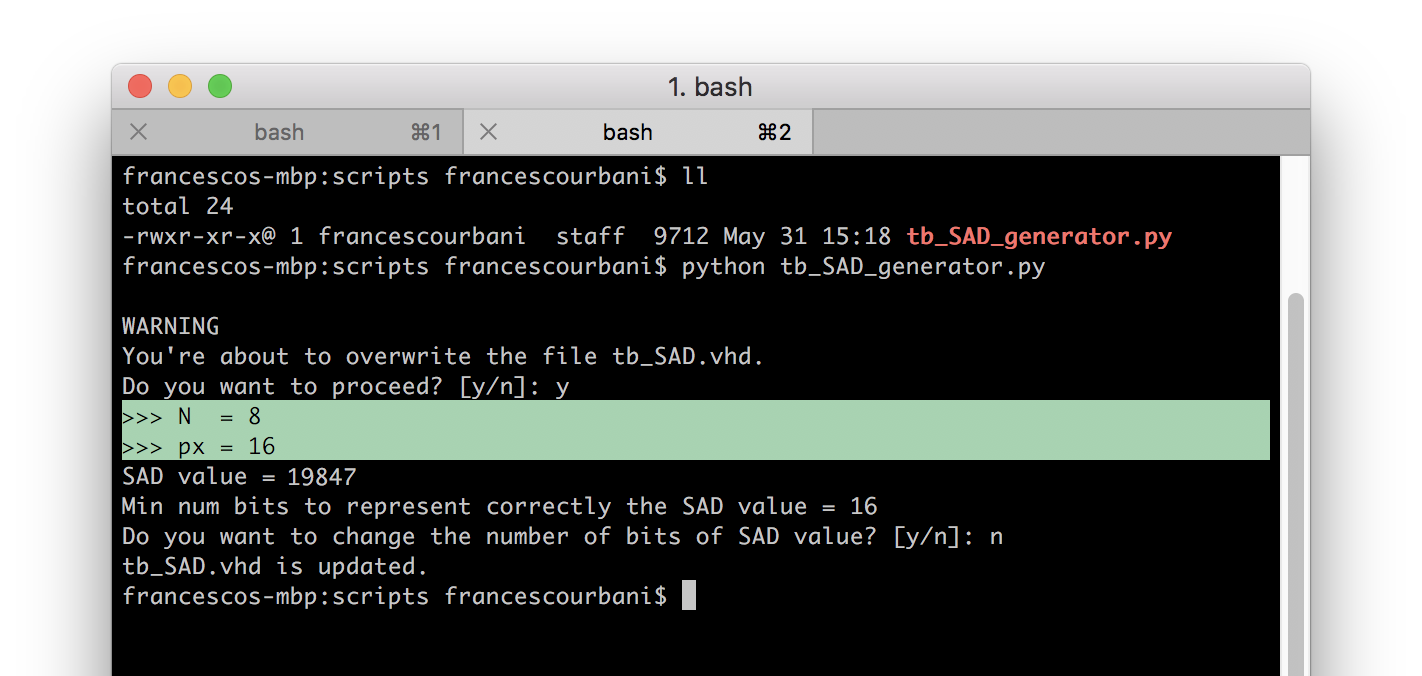
\includegraphics[scale=0.5]{../screenshots/gtkwave/sim1_term.png}
\caption{Test bench generation, first simulation}%\label{fig:7}
\end{figure}


\begin{figure}[h!]
%\centering
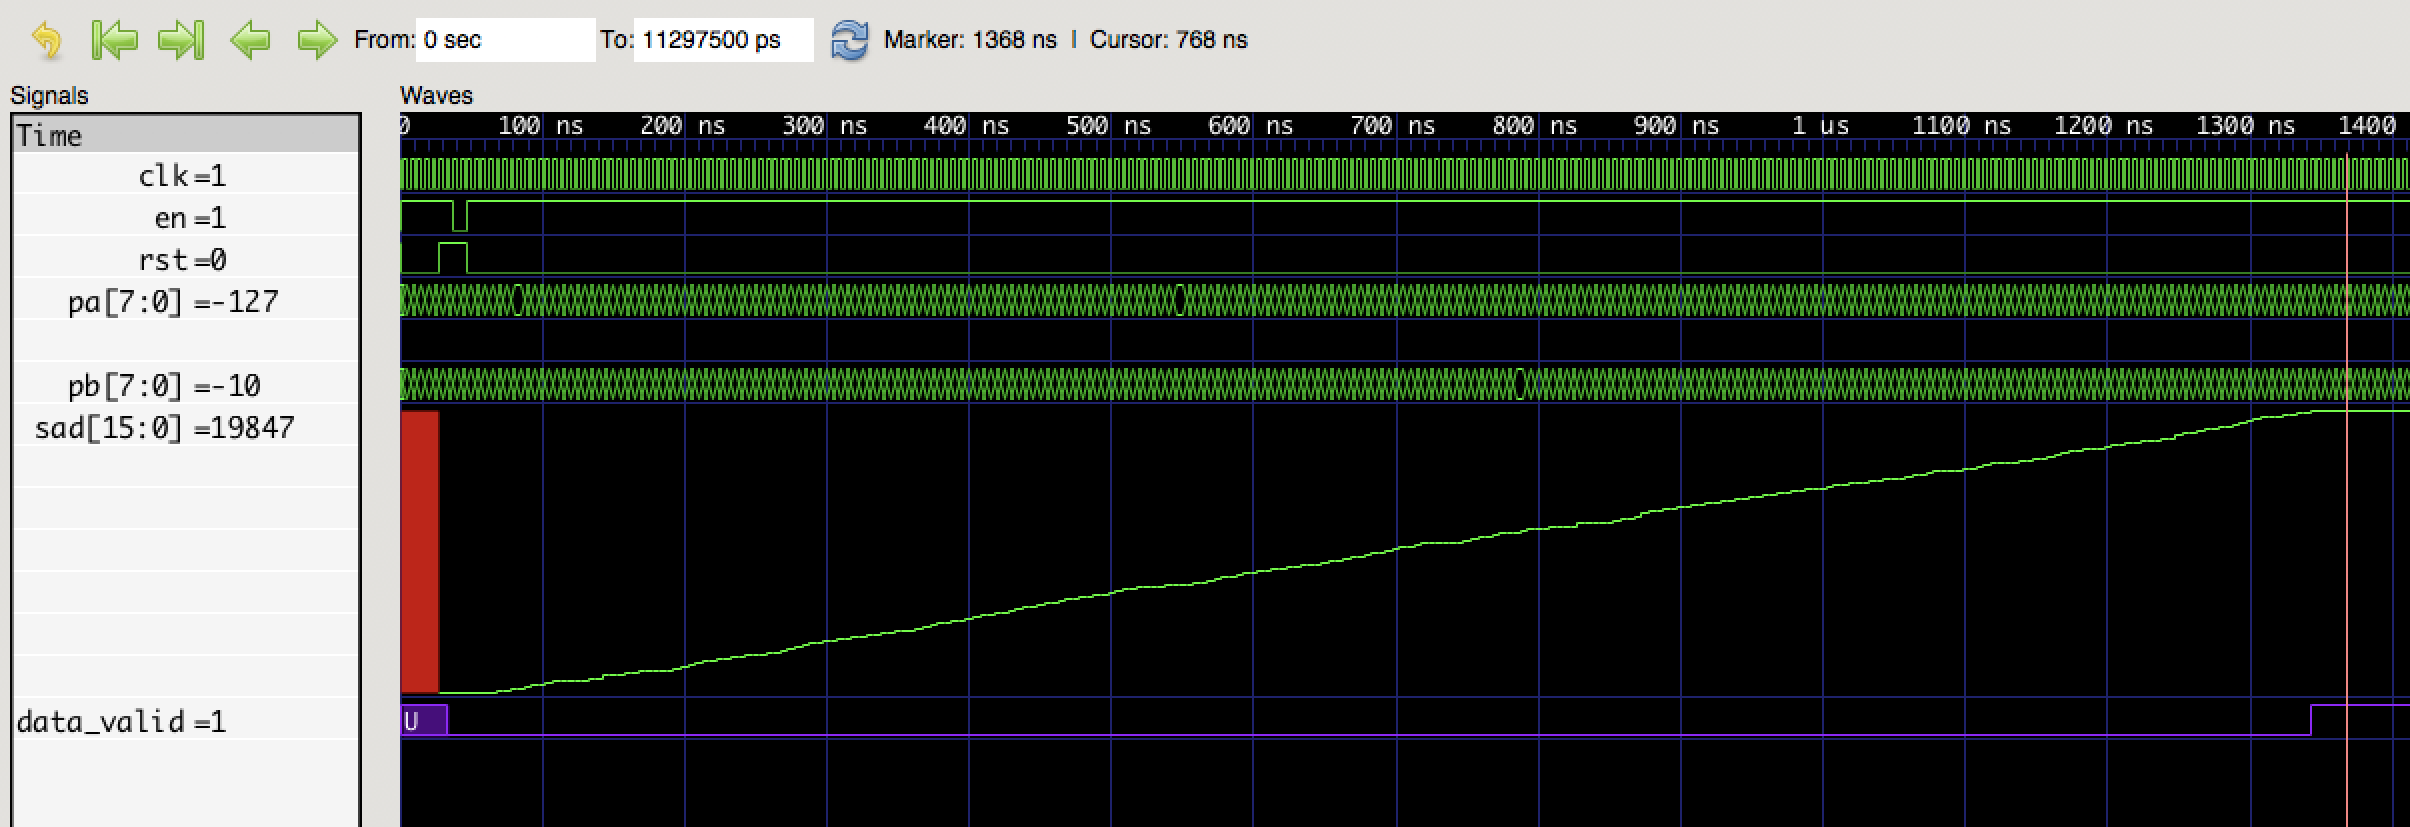
\includegraphics[scale=0.18]{../screenshots/gtkwave/sim1_gtkwave.png}
\caption{Waveform result, first simulation.}\label{fig:wave1}
\end{figure}

We can see from fig. \ref{fig:wave1} that when \texttt{data\_valid} is set, \texttt{sad[15:0]} corresponds to the expected value given by the script.


\begin{figure}[h!]
%\centering
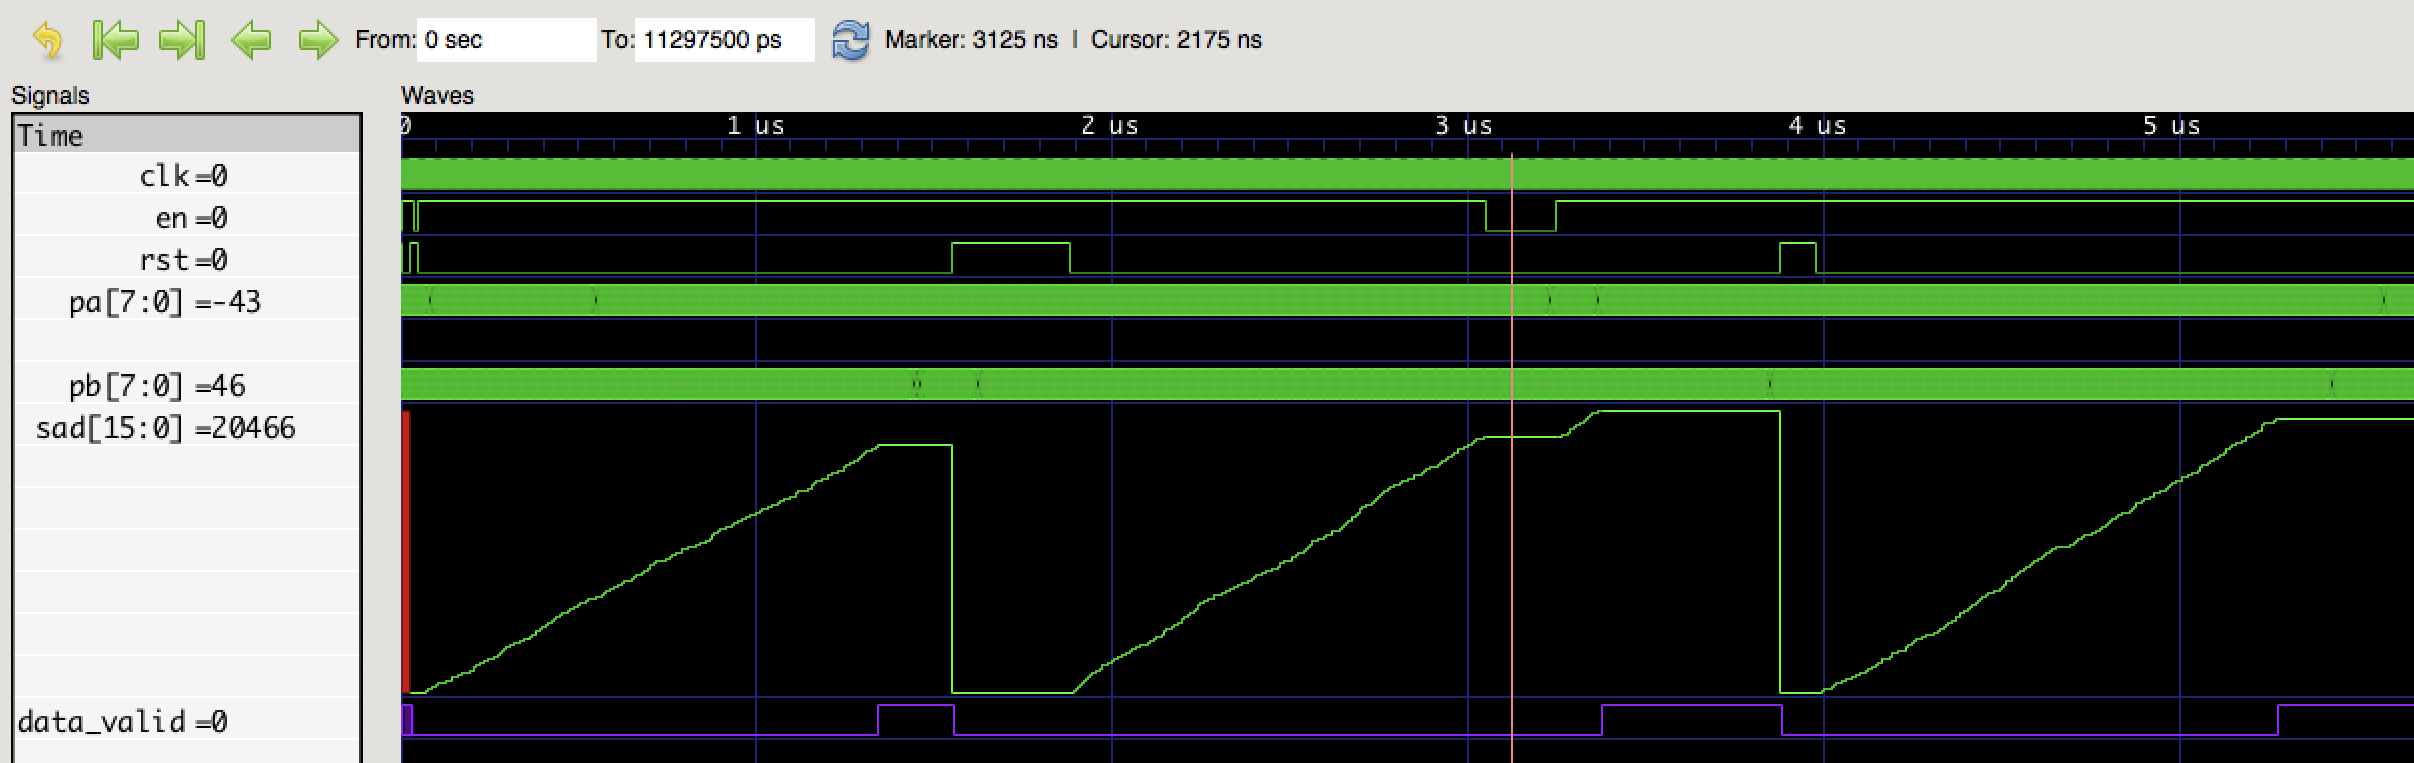
\includegraphics[scale=0.18]{../screenshots/gtkwave/sim1_gtkwave2.png}
\caption{Waveform result, first simulation, unzoomed}\label{fig:wave2}
\end{figure}


We can see from fig. \ref{fig:wave2} that when \texttt{en} is 0, the SAD value does not increase, nor creates a discontinuity when the system resumes its operation, meaning that the state of the system does not change, as requested by the specs. 
This is due to the fact that the \textit{enable} signal in its low state also resets the two input PIPO registers, preventing them from processing their inputs.

If this was not specifically planned, even though the \textit{SAD} output would be frozen, the system would still be internally processing the inputs coming in, and creating a sort of discontinuity of the output signal \textit{SAD} when the system would resume to it's normal operational state.




%\newpage

\subsection{Simulation 2}

Inputs: \texttt{N}=10; \texttt{px}=11. Number of bits to correctly store \texttt{SAD}=17.

\begin{figure}[h!]
%\centering
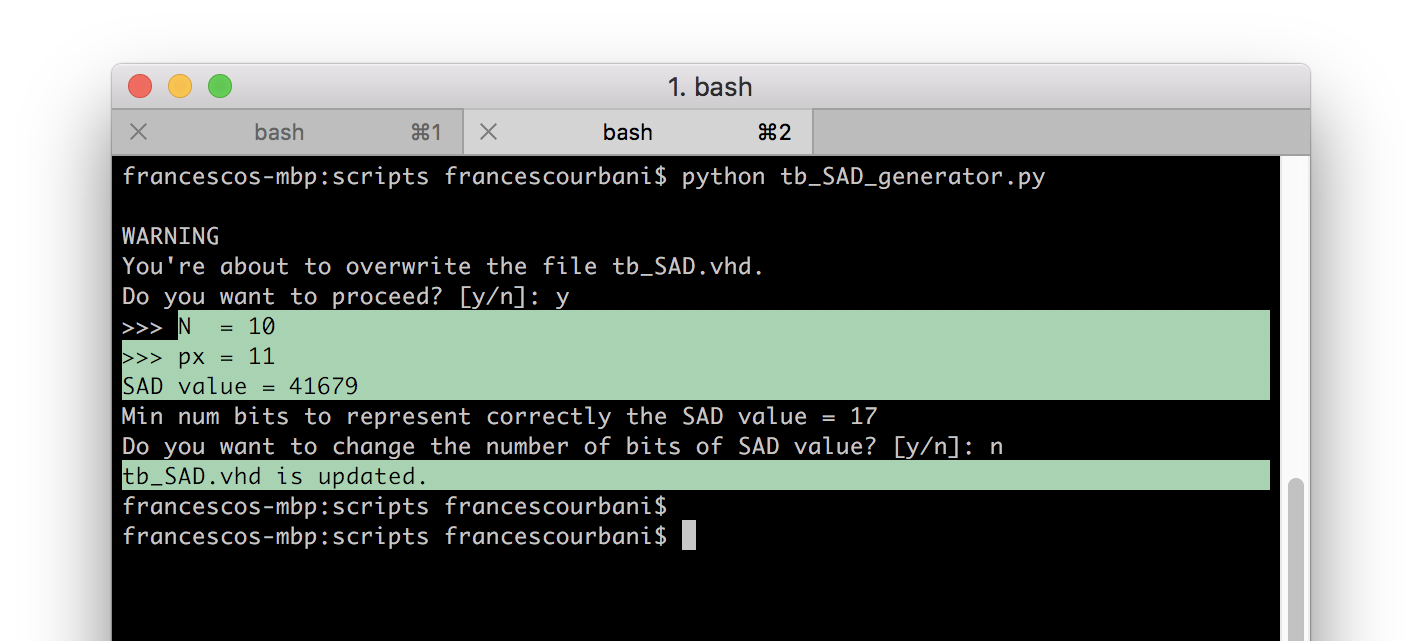
\includegraphics[scale=0.5]{../screenshots/gtkwave/sim2_term.png}
\caption{Test bench generation, second simulation}\label{fig:term2}
\end{figure}



\begin{figure}[h!]
%\centering
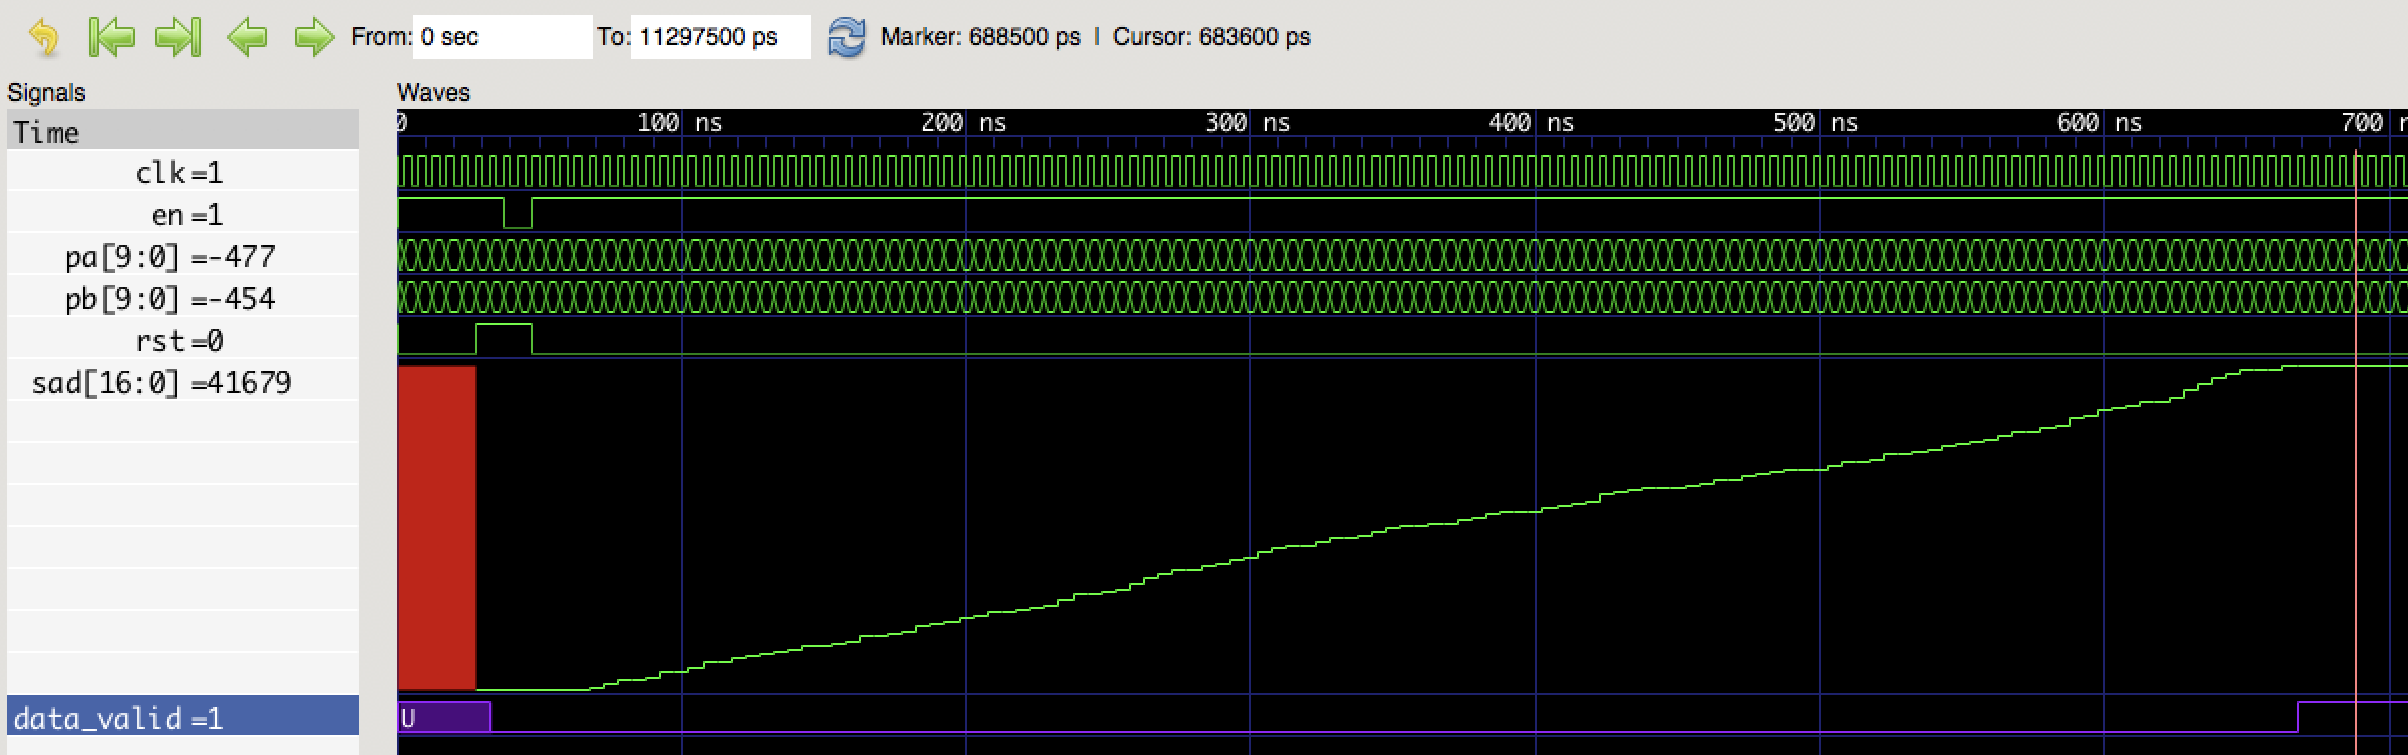
\includegraphics[scale=0.18]{../screenshots/gtkwave/sim2_gtkwave.png}
\caption{Waveform result, second simulation.}\label{fig:wave3}
\end{figure}

Again, we can see (fig. \ref{fig:term2}) that changing the input parameters leads to a re-adaptation the number of bits to correctly store \textit{SAD}, which turns out to be 17 with these two input values. 

The results match.


\newpage

\subsection{Simulation 3}
Inputs: \texttt{N}=8; \texttt{px}=16.

This is actually the dummy simulation made beforehand to check some preliminary results. 

We can see that leaving the two inputs \texttt{pa[7:0]} and \texttt{pb[7:0]} unchanged and fixed, respectively, at \texttt{1} and \texttt{0}, leads to a SAD value, once complete, of \texttt{256} which is actually the total number of pixels given as input, ($\texttt{px}^2$).




\begin{figure}[h!]
%\centering
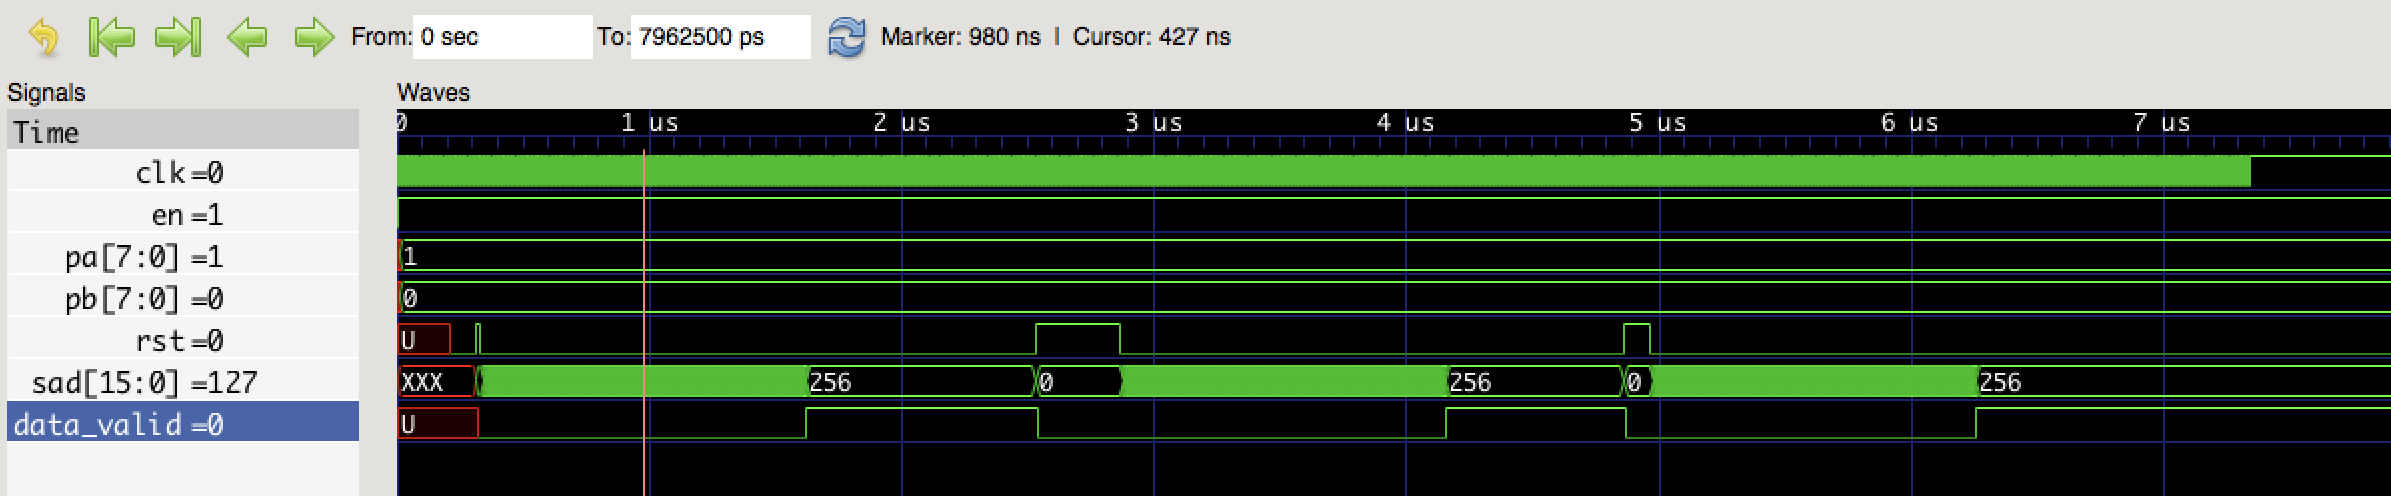
\includegraphics[scale=0.18]{../screenshots/gtkwave/sim3_gtkwave.png}
\caption{Waveform result, third simulation.}%\label{fig:7}
\end{figure}



\newpage







\section{Synthesis and implementation}

I will now walk through the synthesis and implementation of my design onto the Xilinx Zynq-7000 \texttt{xc7z010clg400-1} FPGA, through it's proprietary HDL design suite \href{https://www.xilinx.com/products/design-tools/vivado.html}{Vivado}.
\newline

What matter most at this point of the design is evaluating the maximum clock speed that the system is able to reach reliably, along with the critical path, the power consumption and the resources utilization.

After setting a clock period of 6 ns (i.e. 167 MHz) as time constraint for the synthesis and implementation engines, we can now analyze the results given by the tool.
\newline

This is the compact \textit{Project Summary} that Vivado provides after the synthesis and implementation are successfully executed, (\textit{timing constraints are met}).






\begin{figure}[h!]
\centering
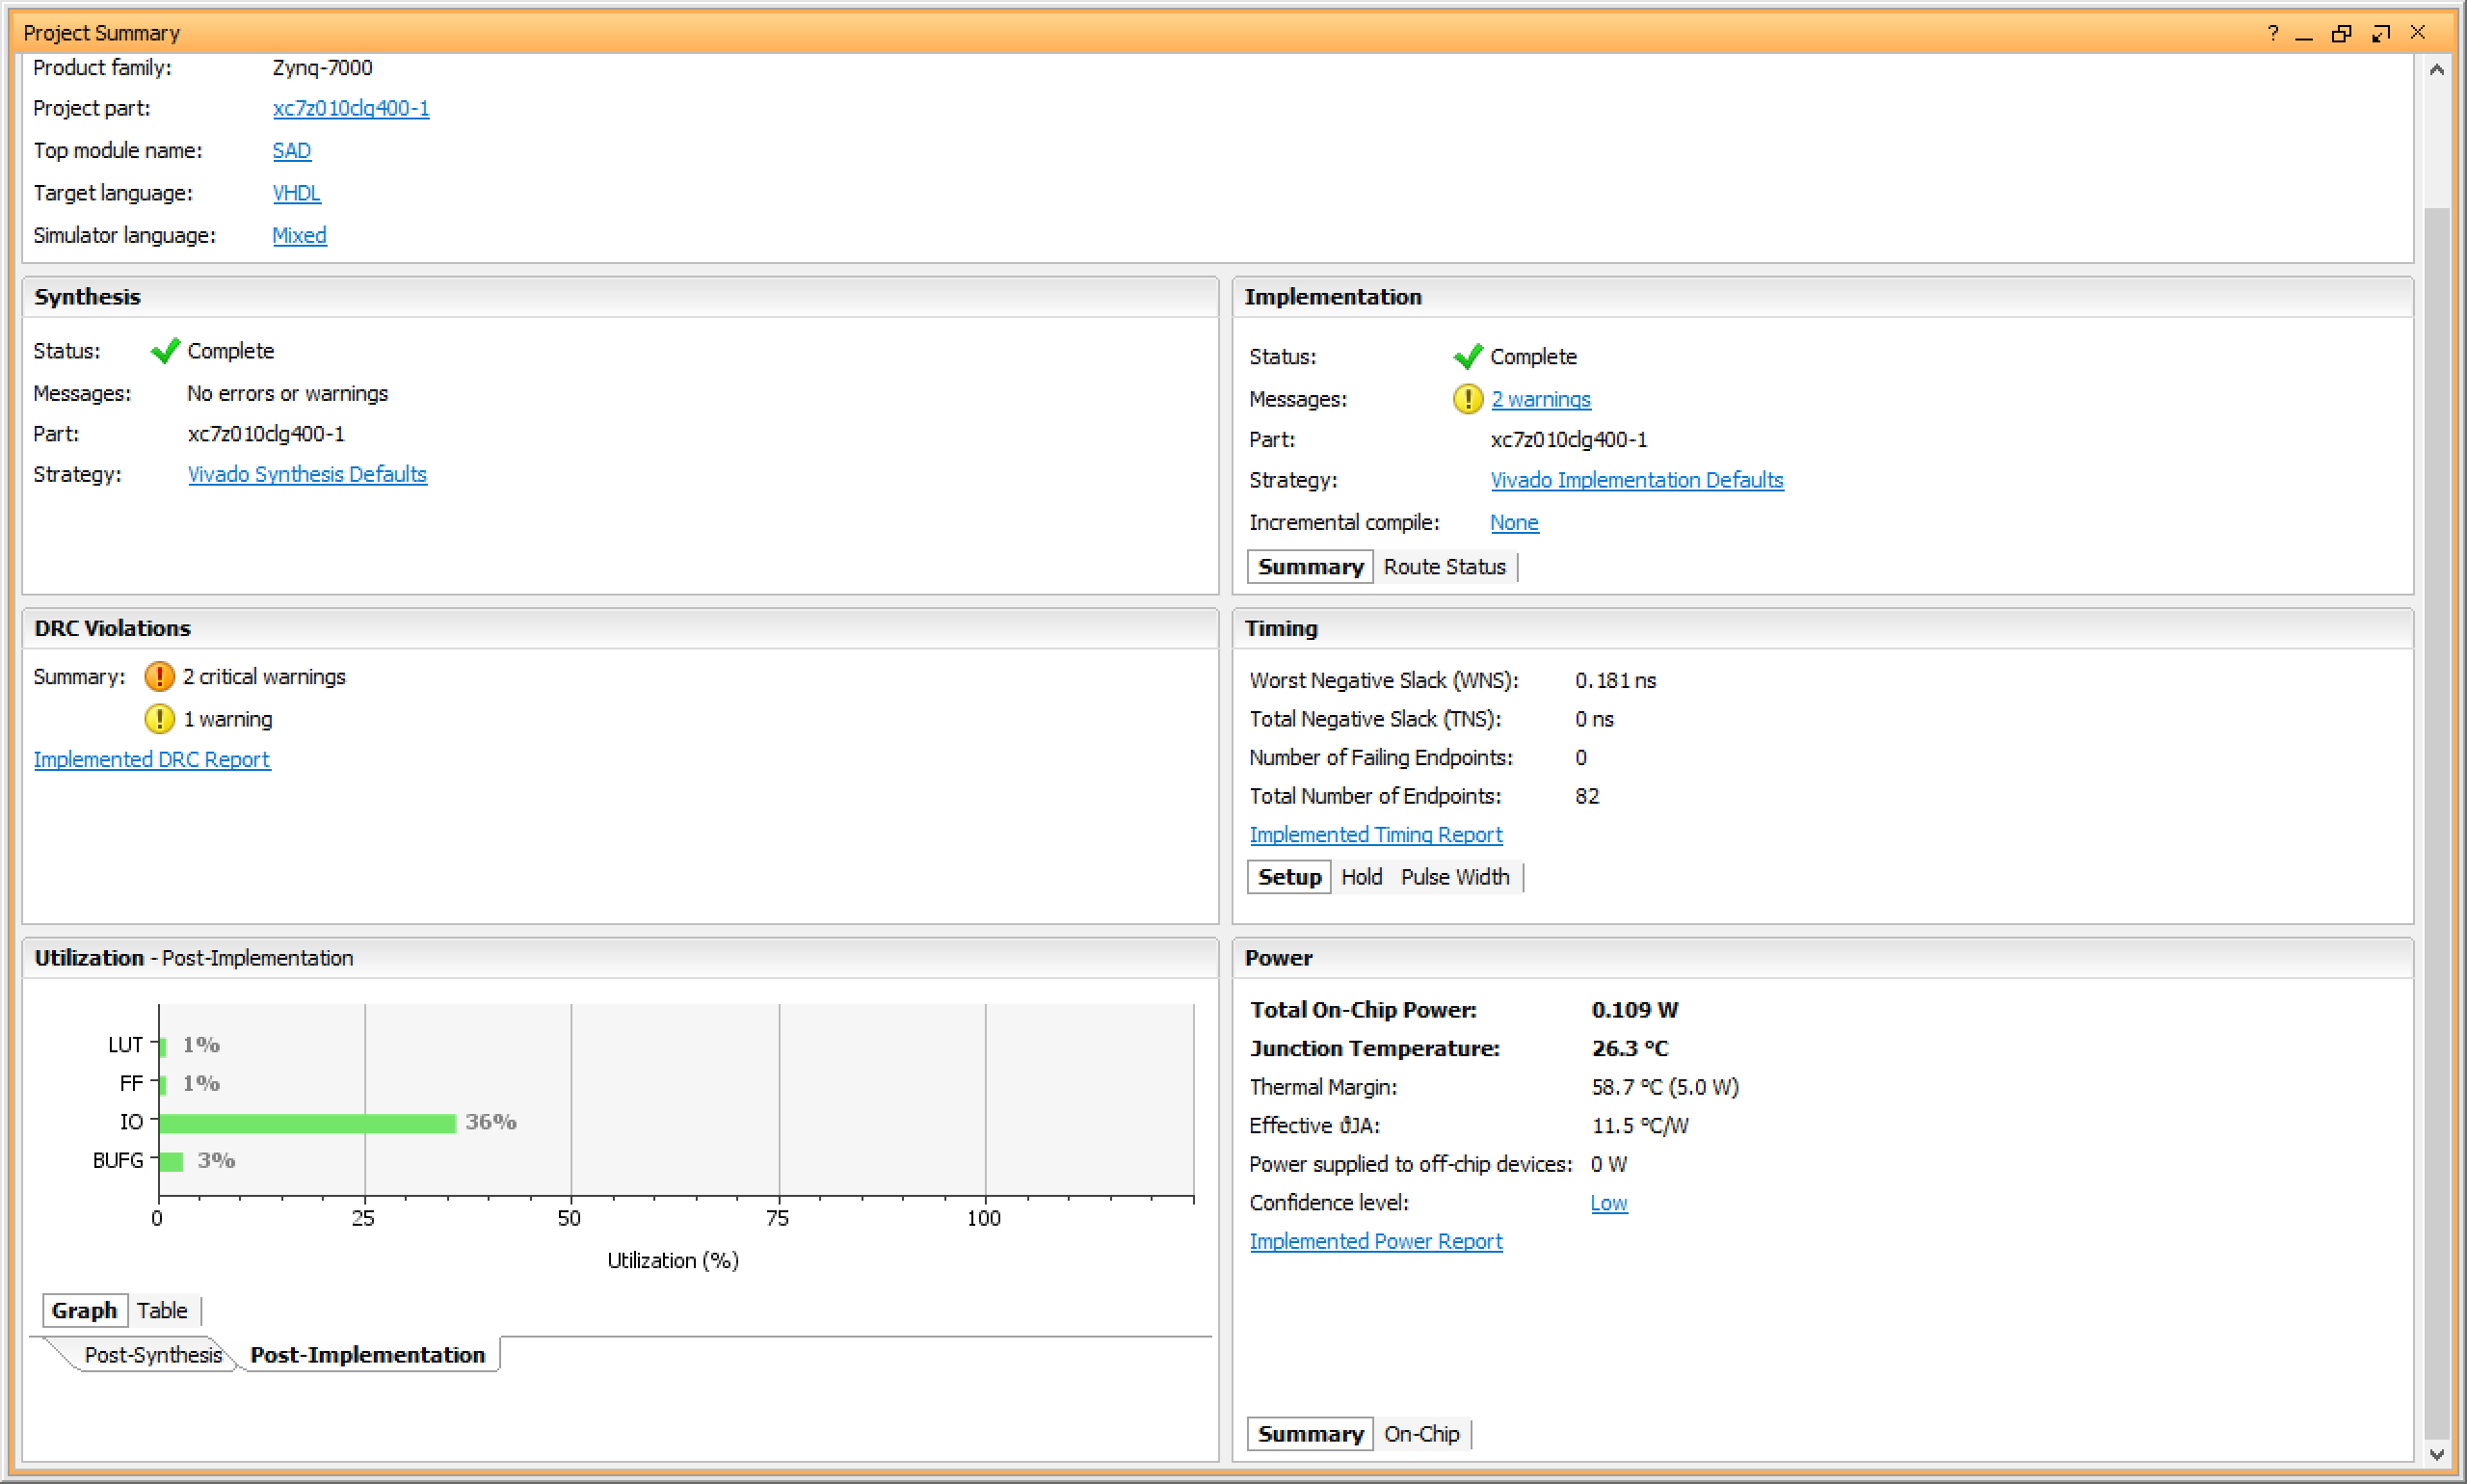
\includegraphics[scale=0.4]{../screenshots/vivado/project_summary.png}
\caption{Vivado Project Summary}%\label{fig:7}
\end{figure}



\bigskip
\bigskip
In order to gain even more detailed information and have a deeper understanding of what's going on, some Tcl commands have been issued to the Vivado Tcl console:
\newline

\begin{itemize}

\item \texttt{report\_utilization -file rpt\_utilization.rpt} to generate a resources utilization report and store it into a file;

\item \texttt{report\_timing\_summary -file rpt\_timing\_summary.rpt} to generate timing report and store it into a file;

\item \texttt{report\_power -file rpt\_power.rpt} to generate a power consumption report and store it into a file;

\item \texttt{report\_route\_status -file rpt\_route\_status.rpt} 

\item \texttt{report\_clock\_interaction -file rpt\_clk\_interaction.rpt}

\item \texttt{report\_clock\_networks -file rpt\_clk\_networks.rpt}

\end{itemize}



and got all these files automatically saved into the folder \texttt{./vivado/SAD} to be opened and read via a text editor.

\subsection{Utilization report}
What's worth highlighting about the content of the file \texttt{rpt\_utilization.rpt} is:



\begin{Verbatim}

1. Slice Logic
--------------

+-------------------------+------+-------+-----------+-------+
|        Site Type        | Used | Fixed | Available | Util% |
+-------------------------+------+-------+-----------+-------+
| Slice LUTs              |   56 |     0 |     17600 |  0.32 |
|   LUT as Logic          |   56 |     0 |     17600 |  0.32 |
|   LUT as Memory         |    0 |     0 |      6000 |  0.00 |
| Slice Registers         |   83 |     0 |     35200 |  0.24 |
|   Register as Flip Flop |   83 |     0 |     35200 |  0.24 |
|   Register as Latch     |    0 |     0 |     35200 |  0.00 |
| F7 Muxes                |    0 |     0 |      8800 |  0.00 |
| F8 Muxes                |    0 |     0 |      4400 |  0.00 |
+-------------------------+------+-------+-----------+-------+





2. Slice Logic Distribution
---------------------------

+-------------------------------------------+------+-------+-----------+-------+
|                 Site Type                 | Used | Fixed | Available | Util% |
+-------------------------------------------+------+-------+-----------+-------+
| Slice                                     |   35 |     0 |      4400 |  0.80 |
|   SLICEL                                  |   24 |     0 |           |       |
|   SLICEM                                  |   11 |     0 |           |       |
| LUT as Logic                              |   56 |     0 |     17600 |  0.32 |
|   using O5 output only                    |    0 |       |           |       |
|   using O6 output only                    |   26 |       |           |       |
|   using O5 and O6                         |   30 |       |           |       |
| LUT as Memory                             |    0 |     0 |      6000 |  0.00 |
|   LUT as Distributed RAM                  |    0 |     0 |           |       |
|   LUT as Shift Register                   |    0 |     0 |           |       |
| LUT Flip Flop Pairs                       |   29 |     0 |     17600 |  0.16 |
|   fully used LUT-FF pairs                 |   15 |       |           |       |
|   LUT-FF pairs with one unused LUT output |   14 |       |           |       |
|   LUT-FF pairs with one unused Flip Flop  |   14 |       |           |       |
| Unique Control Sets                       |    4 |       |           |       |
+-------------------------------------------+------+-------+-----------+-------+

\end{Verbatim}

which shows that the device is mostly unutilized, as we can also see from the \textit{device view} (fig \ref{fig:deviceview}).




\begin{figure}[h!]
\centering
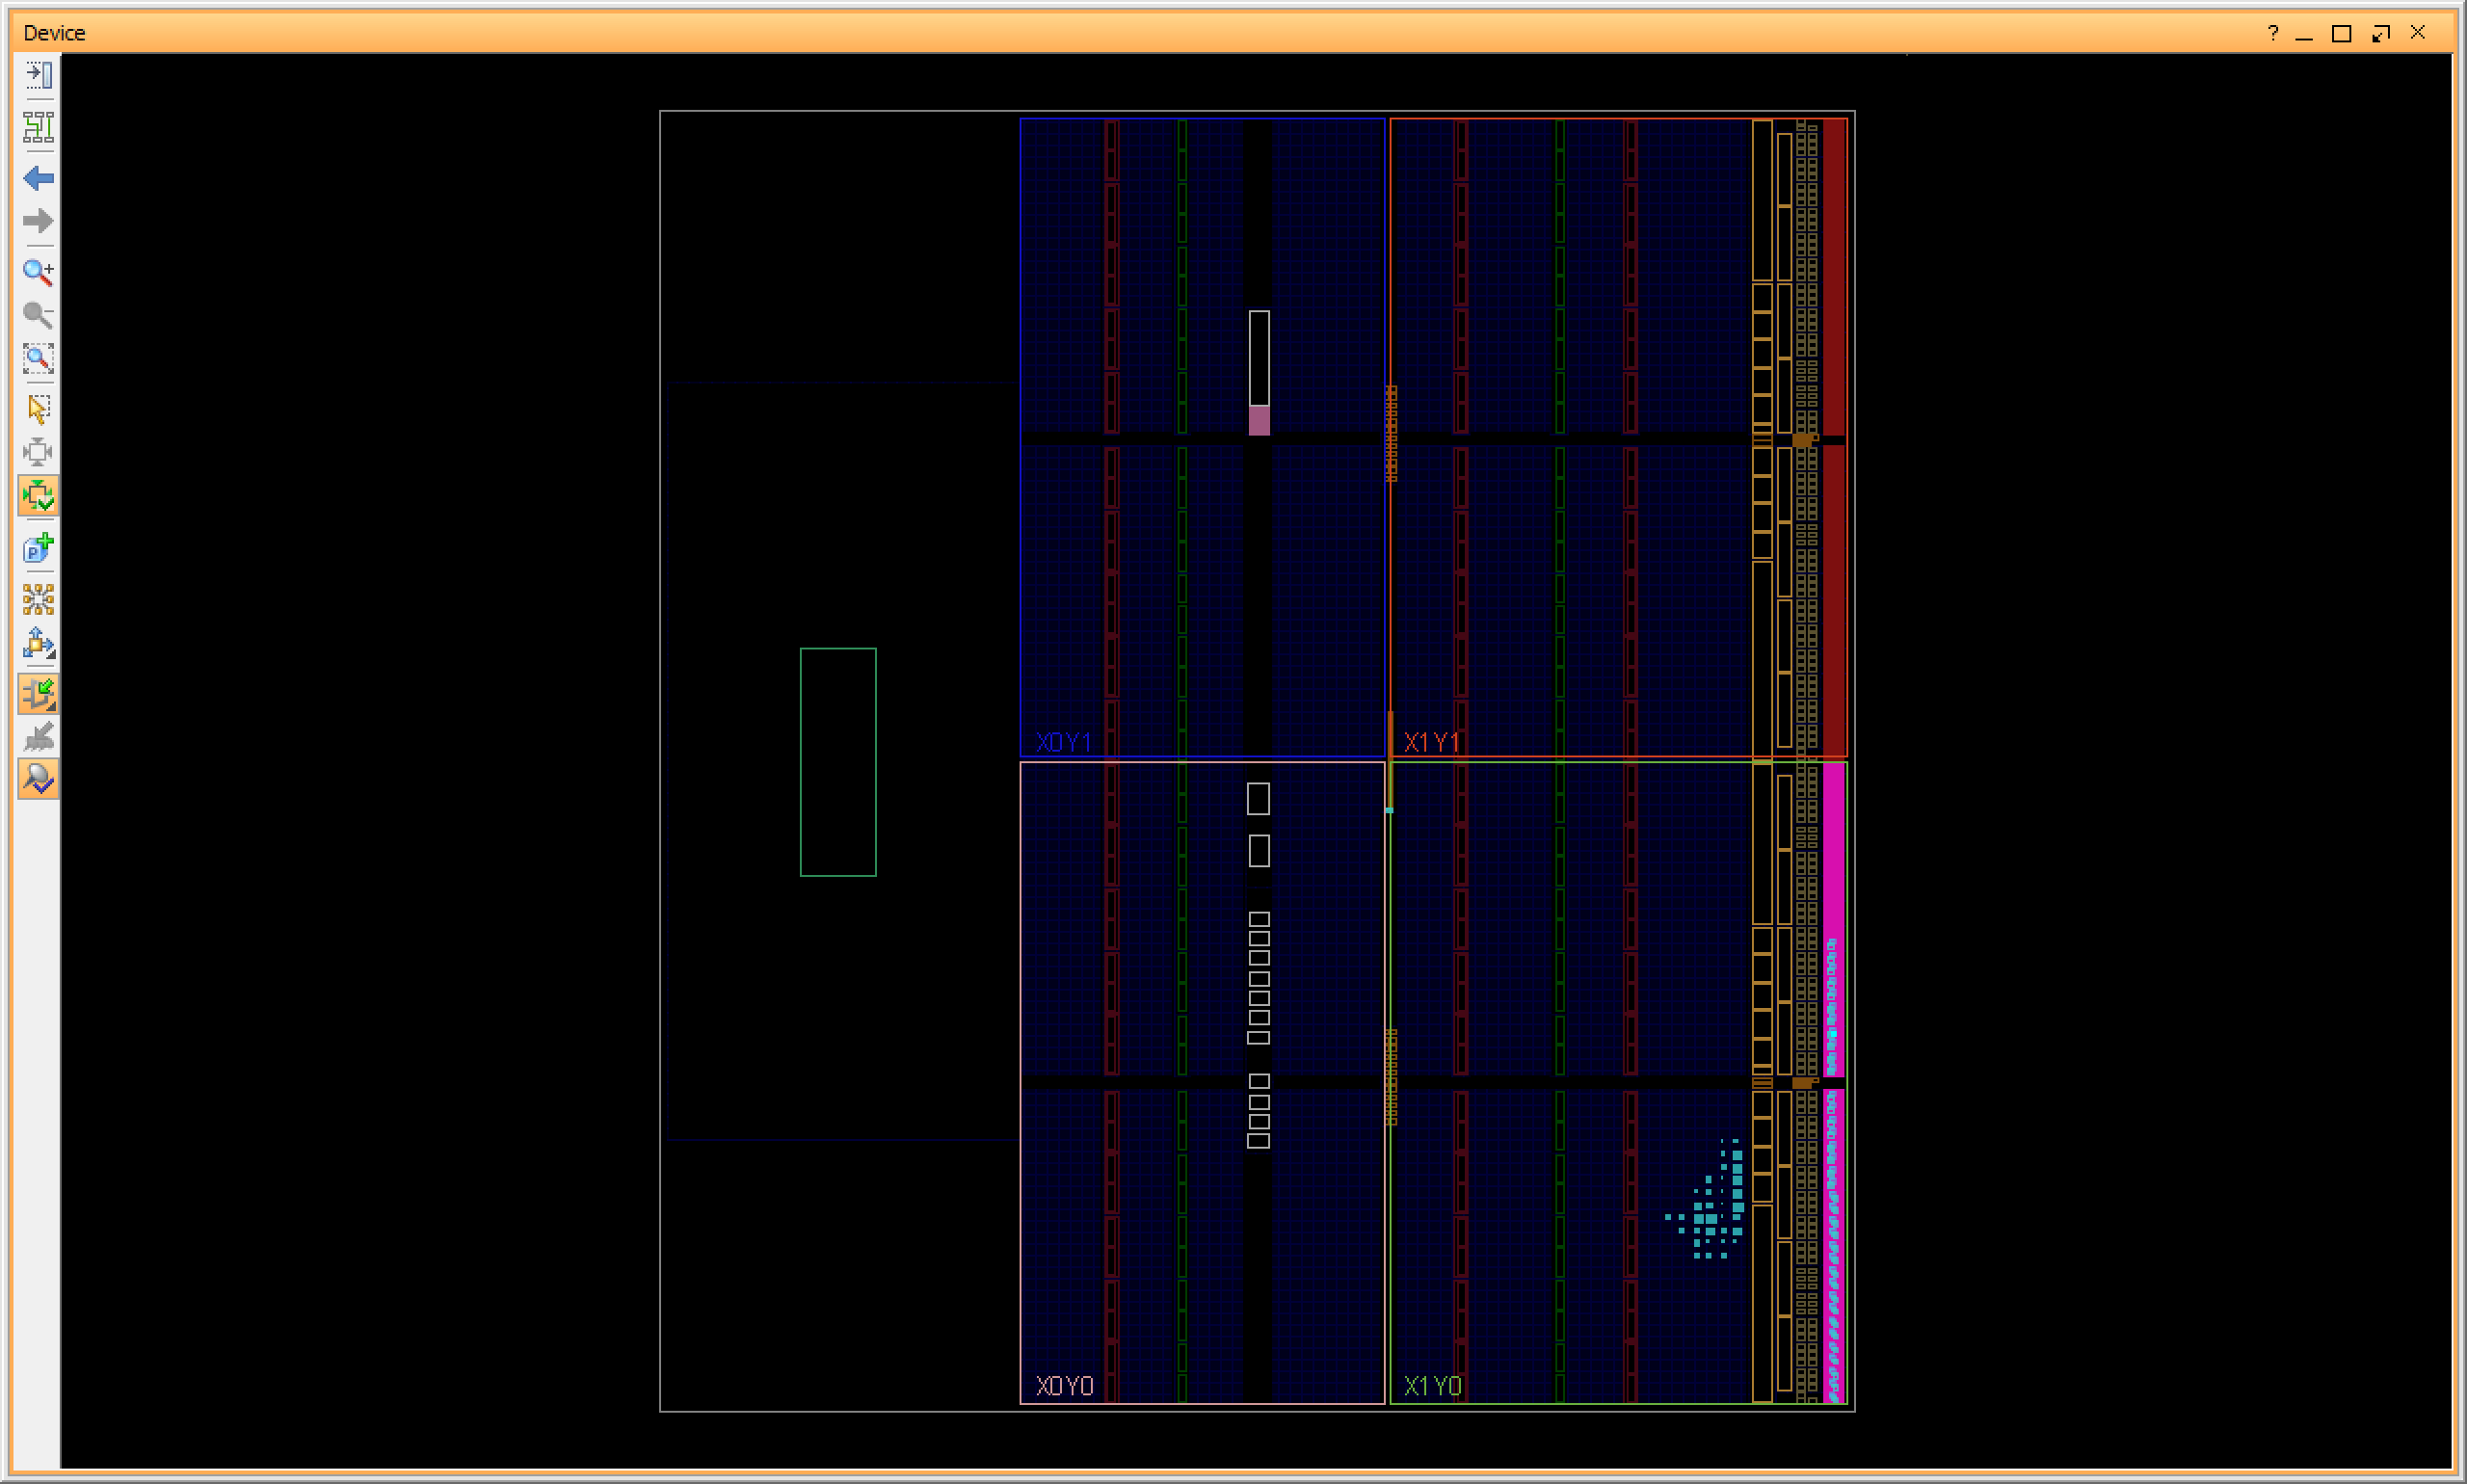
\includegraphics[scale=0.4]{../screenshots/vivado/device.png}
\caption{Vivado, device view}\label{fig:deviceview}
\end{figure}





\newpage
\subsection{Timing summary report}

Let's now open \texttt{rpt\_timing\_summary.rpt}


\begin{Verbatim}[commandchars=\\\{\}]
    

Max Delay Paths
--------------------------------------------------------------------------------------
Slack \textcolor{red}{(MET) :             0.181ns}  (required time - arrival time)
  Source:                 reg_PB/reg_gen[3].i_dff/q_reg/C
                            (rising edge-triggered cell FDCE clocked by clk_6ns  {rise@0.000ns fall@3.000ns period=6.000ns})
  Destination:            phaseacc/i_reg/reg_gen[13].i_dff/q_reg/D
                            (rising edge-triggered cell FDCE clocked by clk_6ns  {rise@0.000ns fall@3.000ns period=6.000ns})
  Path Group:             \textcolor{red}{clk_6ns}
  Path Type:              Setup (Max at Slow Process Corner)
  Requirement:            \textcolor{red}{6.000ns } (clk_6ns rise@6.000ns - clk_6ns rise@0.000ns)
  \textcolor{red}{Data Path Delay:        5.755ns  (logic 2.498ns (43.403%)  route 3.257ns (56.597%))}
  Logic Levels:           8  (CARRY4=2 LUT3=1 LUT4=2 LUT5=2 LUT6=1)
  Clock Path Skew:        -0.060ns (DCD - SCD + CPR)
    Destination Clock Delay (DCD):    4.455ns = ( 10.455 - 6.000 ) 
    Source Clock Delay      (SCD):    4.970ns
    Clock Pessimism Removal (CPR):    0.455ns
  Clock Uncertainty:      0.035ns  ((TSJ^2 + TIJ^2)^1/2 + DJ) / 2 + PE
    Total System Jitter     (TSJ):    0.071ns
    Total Input Jitter      (TIJ):    0.000ns
    Discrete Jitter          (DJ):    0.000ns
    Phase Error              (PE):    0.000ns
--------------------------------------------------------------------------------------
\end{Verbatim}


The key part of these lines are those red-highlighted.

The requirement was 6 ns and the slack 0.181 ns (note that it’s positive), which means that we could have asked for a clock period 0.181 ns shorter and it would still be OK. So it could have been $(6– 0.181)$ ns $ = 5.819$ ns, which is 172 MHz.

The answer to what's the maximum frequency is then 172 MHz, but this value could change if the constraints change.

The Data Path Delay tells us something about what made this worst path slow, how much delay went on logic, and how much on the (estimated) route delays. So does the detailed delay report that follows.
\newline

Note that this is the Max Delay Paths section, there is also a Min Delay Paths section which is useful for spotting hold time violation, and has no effect on the maximum frequency.


%\subsection{Route status report}

%\begin{Verbatim}

%Design Route Status
%                                               :      # nets :
%   ------------------------------------------- : ----------- :
%   # of logical nets.......................... :         275 :
%       # of nets not needing routing.......... :         104 :
%           # of internally routed nets........ :         104 :
%       # of routable nets..................... :         171 :
%           # of fully routed nets............. :         171 :
%       # of nets with routing errors.......... :           0 :
%   ------------------------------------------- : ----------- :



%\end{Verbatim}


\subsection{Power consumption report}

The following piece from the file \texttt{rpt\_power.rpt} reports who needs most power on the chip, differentiate between static and dynamic and estimate whether a heat sink is required for the application or not.

\begin{Verbatim}[commandchars=\\\{\}]


1. Summary
----------

+--------------------------+-------+
| \textcolor{red}{Total On-Chip Power (W)  | 0.109} |
| Dynamic (W)              | 0.007 |
| Device Static (W)        | 0.102 |
| Effective TJA (C/W)      | 11.5  |
| Max Ambient (C)          | 83.7  |
| Junction Temperature (C) | 26.3  |
| Confidence Level         | Low   |
| Setting File             | ---   |
| Simulation Activity File | ---   |
| Design Nets Matched      | NA    |
+--------------------------+-------+


1.1 On-Chip Components
----------------------

+----------------+-----------+----------+-----------+-----------------+
| On-Chip        | Power (W) | Used     | Available | Utilization (%) |
+----------------+-----------+----------+-----------+-----------------+
| Clocks         |     0.001 |        3 |       --- |             --- |
| Slice Logic    |    <0.001 |      219 |       --- |             --- |
|   LUT as Logic |    <0.001 |       60 |     17600 |            0.34 |
|   Register     |    <0.001 |       83 |     35200 |            0.24 |
|   CARRY4       |    <0.001 |       11 |      4400 |            0.25 |
|   Others       |     0.000 |       39 |       --- |             --- |
| Signals        |    <0.001 |      167 |       --- |             --- |
| I/O            |     0.004 |       36 |       100 |           36.00 |
| Static Power   |     0.102 |          |           |                 |
| Total          |     0.109 |          |           |                 |
+----------------+-----------+----------+-----------+-----------------+


\end{Verbatim}





\newpage


\begin{appendices}

\section{Source code}\label{appendix:code}

This is the source code for the top-level component \texttt{SAD.vhd}. This is also stored into the folder \texttt{./src} together with the other components used. Head over that folder for a mode detailed reference.


\begin{lstlisting}[language=vhdl]


---------------------------------------------
-- Title       : SAD
-- Project     : Final project: SAD Calculation
---------------------------------------------
-- File        : SAD.vhd
-- Language    : VHDL
-- Author(s)   : Francesco Urbani
-- Company     : 
-- Created     : Fri May 18 16:23:33 CEST 2018
---------------------------------------------
-- Description : Actual SAD calculator (top level)
---------------------------------------------
-- Update      :
---------------------------------------------


library ieee;
use ieee.std_logic_1164.all;
-- use ieee.std_logic_unsigned.all;
use ieee.numeric_std.all;



entity SAD is
	generic (
		Npixel     :     positive := 16;                    -- total # of pixels of the image
		Nbit       :     positive := 8;                     -- # bits needed to represent the value of each pixel
		SAD_bits   :     positive := 16                     -- # of bits needed to represent the output
	);
	port (
		CLK        : in  std_logic;	                        -- CLK, active on rising edge
		RST        : in  std_logic;	                        -- RST, active high
		PA         : in  std_logic_vector(Nbit-1 downto 0);	-- input pixel value image A
		PB         : in  std_logic_vector(Nbit-1 downto 0);	-- input pixel value image B
		EN         : in  std_logic;	                        -- enable input

		SAD        : out std_logic_vector(SAD_bits-1 downto 0);	-- ouput SAD value
		DATA_VALID : out std_logic	                        -- specifies whether the output SAD is valid or not
	);
end entity SAD;


architecture struct of SAD is
	
	-- DECLARING COMPONENTS NEEDED.
	component PIPOreg is
		generic (N : positive); -- N BITS PIPO REGISTER
		port (
			clk     : in  std_logic;
			rst     : in  std_logic;
			d       : in  std_logic_vector(N-1 downto 0);
			q       : out std_logic_vector(N-1 downto 0)
		);
	end component;

	component PhaseAccumulator is
		generic (N : positive );
		port(
			clk    : in  std_logic;
			rst    : in  std_logic;
			pa_in  : in  std_logic_vector(N-1 downto 0);
			pa_out : out std_logic_vector(N-1 downto 0)
		);
	end component;


	component counter is
		generic ( overflow_val : natural );
		port (
			count_puls   : in std_logic;
			count_enable : in std_logic;
			rst          : in std_logic;
			tc           : out std_logic
		);
	end component;

	component subtractor is
		generic (Nbit : positive);
		port (
			a : in  std_logic_vector(Nbit-1 downto 0);
			b : in  std_logic_vector(Nbit-1 downto 0);
			s : out std_logic_vector(Nbit-1 downto 0) 
		);
	end component;


	component mux2to1 is
		generic (Nbit : in positive );
		port (
			i0   : in  std_logic_vector(Nbit-1 downto 0);
			i1   : in  std_logic_vector(Nbit-1 downto 0);
			s    : in  std_logic;
			f    : out std_logic_vector(Nbit-1 downto 0)
		) ;
	end component ;

	component SISOreg is
		generic (N  : positive );
		port (
			SI   : in std_logic;
			clk  : in std_logic;
			rst  : in std_logic;
			SO   : out std_logic
		);

	end component;



	-- intermediate signals
	signal padding               : std_logic_vector(SAD_bits-Nbit-1 downto 0); 
                                   -- turns the signal out off the subractor to a number of bits 
                                   -- coherent with the downstream signal

	signal PA_to_sub_nbit        : std_logic_vector(Nbit-1 downto 0);          
                                   -- connection from the out of the reg on the PA side to the subtractor

	signal PB_to_sub_nbit        : std_logic_vector(Nbit-1 downto 0);          
                                   -- connection from the out of the reg on the PB side to the subtractor

	signal sub_out_nbits         : std_logic_vector(Nbit-1 downto 0); 
                                   -- signal out of the subtractor (Nbit)

	signal pa_in                 : std_logic_vector(SAD_bits-1 downto 0);
                                   -- input to the phase accumulator
	
	signal counter_in            : std_logic; 
                                   -- input to the counter enable pin

	signal pa_out                : std_logic_vector(SAD_bits-1 downto 0); 
                                   -- phase accumulator output wire
	
	signal mux_to_reg_out_wire   : std_logic_vector(SAD_bits-1 downto 0);
                                   -- connection from the multiplex to the output PIPO register
	
	signal rst_input_registers   : std_logic;
                                   -- reset input signal to the two heading PIPO registers

	signal sad_wire              : std_logic_vector(SAD_bits-1 downto 0); 
                                   -- output-register output (i.e. the actual SAD signal)
	
	signal tc_wire               : std_logic; -- output of the counter
	signal hold_wire             : std_logic; -- input to the MUX control signal. 
	                                          -- it also coincides with DATA_VALID


begin
		
	rst_input_registers <= EN nand (not RST);
	hold_wire           <= EN nand (not tc_wire);



	reg_PA : PIPOreg
		generic map(Nbit)
		port map (CLK, rst_input_registers, PA, PA_to_sub_nbit);

	reg_PB : PIPOreg
		generic map(Nbit)
		port map (CLK, rst_input_registers, PB, PB_to_sub_nbit);


	-- generating a bunch of zeros to make the padding.
	gen_padding : for i in 0 to SAD_bits-Nbit-1 generate
		padding(i) <= '0';
	end generate;


	-- merging padding and sub_out_nbits to make a new signal called pa_in
	-- which enters the phase accumlator
	pa_in <= padding & sub_out_nbits;

	-- subtractor instance
	sub: subtractor
		generic map(Nbit)
		port map(PA_to_sub_nbit, PB_to_sub_nbit, sub_out_nbits);

	phaseacc: PhaseAccumulator
		generic map(SAD_bits)
		port map(CLK, RST, pa_in, pa_out);


	-- multiplexer on the output register side. 
	-- Needed to freeze the SAD signal when ENABLE is 0 and when the SAD computation is completed.
	mux1 : mux2to1
		generic map(SAD_bits)
		port map(pa_out, sad_wire, hold_wire, mux_to_reg_out_wire);

	reg_out: PIPOreg
		generic map(SAD_bits)
		port map (CLK, RST, mux_to_reg_out_wire, sad_wire);


	-- SISO register made of 3 D flip-flops. 
	-- Needed to delay the ENABLE signal going into the COUNT_ENABLE of the counter.
	-- This was necessary in order to sync the upper path of the SAD calculation
	-- and the COUNTER.
	siso: SISOreg
		generic map(3)
		port map(EN, CLK, RST, counter_in);


	-- counter instance
	-- it counts up to Npixel * Npixel, after that it sets its output to 1,
	-- hence the DATA_VALID signal of the system is high and the SAD value is frozen.
	cnt: counter
		generic map(Npixel)
		port map(CLK, counter_in, RST, tc_wire);

	
	-- connection of the intermediate signals to the output of the SAD.
	SAD        <= sad_wire;
	DATA_VALID <= tc_wire;

end architecture;


\end{lstlisting}




%\section{asd}\label{appendix:ds}
\end{appendices}





\end{document}

